\section{Backpropagation} \label{sec:backprop}

\subsection{Notation} \label{ss:notationBP}
Diesem Lernalgorithmus liegt eine Kostenfunktion zugrunde. Letztendlich wird analysiert wie sich das Netz momentan für einen Trainingsdatensatz verhält. Wenn das Netz diesen richtig erkennt ist der ausgegebene Fehler gering ansonsten ist er hoch.

Um diesen Fehler in einem mehrschichtigen Netz effizient zu minimieren wird in vielen Fällen der \emph{Backpropagation}-Algorithmus verwendet. Er wurde bereits in den Siebzigerjahren definiert, erlangt jedoch erst im Jahr 1986 mit dem Paper \emph{Learning representations by back-propagating errors} von Rumelhart, Hinton und Williams Bekanntheit.

Im vorherigen Teil habe ich bereits beschrieben was man unter dem Gradientenabstieg versteht und wie dieser auch bei mehrdimensionalen Funktionen (wie zum Beispiel der hierbei betrachteten Kostenfunktion) verwendet werden kann. Es wurde jedoch noch nicht vorgestellt, wie man auf ein mehrschichtiges Netz bezogen, diesen Gradienten überhaupt berechnen und nutzen kann um die Fehler der Trainingsbeispiele zu minimieren.

Gemeinhin wird die Notation, wie sie in Abbildung \ref{fig:weight_not} zu sehen ist, für ein Gewicht verwendet. In Abbildung \ref{fig:biasAct_not} steht das $b^l_j$ für den Schwellwert (\emph{Bias}) am Neuron mit dem Index \emph{j} im Layer mit dem Index \emph{l}. Selbes gilt für die Aktivierung welche mit einem \emph{a} gekennzeichnet wird. Mit den gegebenen Notationen können wir folgende Gleichung für die Aktivierung eines Neurons aufstellen (siehe Gleichung \ref{eq:act}).

\begin{figure}[!htb]
	\centering
	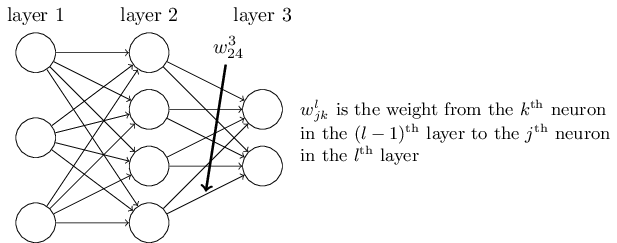
\includegraphics[width=.7\linewidth]{img/weight_notation}
	\mycaption{Notation}{dlnielsen}
	\label{fig:weight_not}
\end{figure}

\begin{figure}[!htb]
	\centering
	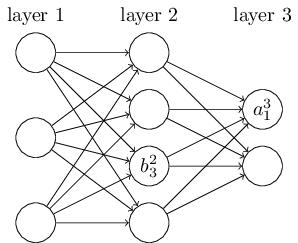
\includegraphics[width=.4\linewidth]{img/biasAct_notation}
	\mycaption{Notation}{dlnielsen}
	\label{fig:biasAct_not}
\end{figure}

\begin{equation} \label{eq:act}
a^{l}_j = \sigma\left( \sum_k w^{l}_{jk} a^{l-1}_k + b^l_j \right),
\end{equation}

Diese Formel sollte bereits aus den vorherigen Kapiteln bekannt sein. Hierbei werden die Gewichte mit den entsprechenden Aktivierungen multipliziert und anschließend aufaddiert. Die generierte Ausgabe wird mit dem Schwellwert verrechnet und in eine Aktivierungsfunktion (z.B. Sigmoid-Funktion) gesteckt.

Um später einfacher mit all diesen Werten zu rechnen wird versucht die gegebenen Werte in eine Matrix- beziehungsweise Vektor-Darstellungsform zu bringen. Da Neuron mehrere ausgehende \myquote{Pfade} besitzen wird hierbei eine Matrix geformt. Das bisher beschriebene Gewicht $w^l_{jk}$ befindet sich hierbei im Zeilenindex \emph{j} und Spaltenindex \emph{k}. Da sich sowohl der Schwellwert als auch die Aktivierung ausschließlich auf ein einzelnes Neuron beziehen, muss hierfür lediglich ein eindimensionaler Vektor pro Layer \emph{l} generiert werden. Die einzelnen Komponenten werden hierbei über den Index \emph{j} angesteuert. Die Notation für den Aktivierungsvektor der Schicht \emph{l} sieht dann derartig aus: $a^l_j$. Ähnliches gilt für die Schwellwerte: $b^l_j$.

Um mit diesen Vektoren arbeiten zu können muss man die abschließende Aktivierungsfunktion $\sigma$ vektorisieren
\footnote{Klarer Verweis auf Nielsen Buch, Kapitel über Backpropagation im Detail \cite{dlnielsen}}.
Dabei muss man die Funktion lediglich derartig umschreiben, dass diese auf die einzelnen Komponenten angewendet wird und nicht auf einen einzelnen Wert. Beispielsweise würde die Funktion $f(x) = x^2$ vektorisiert folgendermaßen aussehen:

\begin{equation}
  f\left(\left[ \begin{array}{c} 2 \\ 3 \end{array} \right] \right)
  = \left[ \begin{array}{c} f(2) \\ f(3) \end{array} \right]
  = \left[ \begin{array}{c} 4 \\ 9 \end{array} \right],
\end{equation}

Mit diesen Zusammenfassungen kann nun die Gleichung \ref{eq:act} folgendermaßen umgeschrieben werden:

\begin{equation}
  a^{l} = \sigma(w^l a^{l-1}+b^l).
\end{equation}

Diese Umschreibung abstrahiert das Denken über die lokalen Neuronen auf ein höheres Level sodass es einfacher ist das Gesamtbild zu betrachten. Um noch mehr Klarheit zu schaffen wird oftmals die Aktivierung einer Schicht \emph{l} aus der Funktion herausgezogen und mit dem Buchstaben \emph{z} versehen. $z^l$ kann nun in die Aktivierungsfunktion $\sigma$ eingesetzt werden. Im folgenden werde ich diese Ausgabewerte, welche in die Aktivierungsfunktion hereingereicht werden, stets mit \emph{z-Wert} abkürzen.

\paragraph{Zusammenfassung} der bisherigen Beschreibungen.

\begin{mytheo}{Backpropagation - Notation}{theoexample}

Bisherige Schreibweise: Komponentenweise Darstellung
\begin{equation}
  a^{l}_j = \sigma\left( \sum_k w^{l}_{jk} a^{l-1}_k + b^l_j \right) \nonumber
\end{equation}

Zusammengefasste Form: Vektorisierte Form
\begin{equation} \label{eq:zusForm}
a^l = \sigma(z^l)
\end{equation}

Gewichtete Eingabe (\emph{Z-Werte}):
\begin{equation} \label{eq:gewEin}
  z^l \equiv w^l a^{l-1}+b^l
\end{equation}

\end{mytheo}

\subsection{Fundamentale Gleichungen}

Ziel des Backpropagation-Algorithmus ist es herauszubekommen welche Gewichte und Schwellwerte verändert werden müssen um die Kostenfunktion zu minimieren. Im folgenden werde ich nach und nach die vier wichtigsten Formeln des Verfahrens beschreiben.

\begin{mytheo}{Backpropagation - Fundamentale Gleichungen}{theoexample} \label{theo:zus}

\begin{equation} \label{eq:error}
\delta^L = \nabla_a C \odot \sigma'(z^L).
\end{equation}

\begin{equation} \label{eq:recError}
\delta^l = ((w^{l+1})^T \delta^{l+1}) \odot \sigma'(z^l),
\end{equation}

\begin{equation} \label{eq:biasError}
\frac{\partial C}{\partial b^l_j} = \delta^l_j.
\end{equation}

\begin{equation} \label{eq:weightError}
\frac{\partial C}{\partial w^l_{jk}} = a^{l-1}_k \delta^l_j.
\end{equation}

\end{mytheo}

% \begin{figure}[!htb]
%	\centering
%
% \Tree [.C \qroof{Label}.y [.$a^{l+1}_j$ [ .$z^{l+1}_j$ [ $w^l_j$ [ .$a^l_j$ [ .$z^l_j$ \qroof{Weight}.$w^l_j$ \qroof{Activation}.$a^{l-1}_j$ \qroof{Bias}.$b^l_j$ ] ] $b^l_j$ ] ] ] ]
%	\caption [Baumdarstellung]{Baumdarstellung - Zusammenhang der Gewichte, Aktivierungen und Schwellwerte \cite{3b1b}}
%	\label{fig:tree}
% \end{figure}

\paragraph{Fehler auf der Ausgabeschicht - Gleichung \ref{eq:error}}
Um zu verstehen was man unter einem Fehler genau versteht sei angenommen die Ausgabe eines Neurons \emph{j} im Layer \emph{l} wird um einen unbestimmten Wert verzerrt. Mathematisch ausgedrückt sieht dies dann folgendermaßen aus:

\begin{equation}
\sigma(z^l_j+\Delta z^l_j)
\end{equation}

Statt der herkömmlichen Ausgabe $\sigma(z^l_j)$ wird ein \emph{Fehler} $\Delta z^l_j$ hinzugefügt. Allgemein wird der Fehler eines einzelnen Neurons dadurch folgendermaßen beschrieben:

\begin{equation}
\delta^l_j \equiv \frac{\partial C}{\partial z^l_j}.
\end{equation}

Fangen wir jedoch von vorne an. Bei der Backpropagation wird versucht von den Fehlern welche am Ende auftreten auf die verschiedenen Gewichte und Schwellwerte zu schließen die verändert werden müssen. Dabei wird zuallererst der durchschnittliche Fehler der letzten Schicht berechnet. Hierfür wird die Kostenfunktion nach dem jeweiligen z-Wert eines Neurons mit Index \emph{j} abgeleitet.

\begin{equation} \label{eq:1}
\delta^L_j = \frac{\partial C}{\partial z^L_j}
\end{equation}

Das \emph{L} steht diesbezüglich für den letzten (Ausgabe-) Layer. Dieser Ausdruck kann etwas verfeinert werden, indem man die Kettenregel anwendet\footnote{Der Youtuber 3blue1brown hat hierzu ein sehr gutes Video produziert welches die Zusammenhänge mit der Kettenregel verdeutlicht \cite{3b1b} (Kapitel: Backpropagation)}. Zur Erinnerung, die Kettenregel sieht folgendermaßen aus:

\begin{equation}
\frac{d}{{dx}}\left[ {f\left( u \right)} \right] = \frac{d}{{du}}\left[ {f\left( u \right)} \right]\frac{{du}}{{dx}}
\end{equation}

Für die Vereinfachung der Gleichung \ref{eq:1} wird die Definition von \emph{z} herangezogen. Wir erinnern uns, $a^l = \sigma(z^l)$ (siehe Gleichung \ref{eq:zusForm}). \emph{z} stellt in diesem Fall den kompletten Ausgabewert des Neurons dar \emph{bevor} dieser in die Aktivierungsfunktion gesteckt wurde und berechnet sich wie schon in Gleichung \ref{eq:gewEin} gezeigt mit ${z^l \equiv w^l a^{l-1}+b^l}$. Wenn man die Kostenfunktion nun nach \emph{z} ableiten möchte, muss man hierbei erst einmal die äußere mit der inneren Ableitung multiplizieren. Es entsteht folgende Gleichung:

\begin{equation}
\delta^L_j = \sum_k \frac{\partial C}{\partial a^L_k} \frac{\partial a^L_k}{\partial z^L_j}
\end{equation}

Da die Aktivierung $a^L_k$ im letzten Term lediglich vom Neuron mit dem Index \emph{k} abhängt bilden alle Summanden mit $k \neq j$ den Wert 0. Es kann folglich auf die nachfolgende Gleichung geschlossen werden. (Dieses Entfallen der Summe war bereits in der Herleitung des Gradientenabstiegs zu beobachten).

\begin{equation}
\delta^L_j = \frac{\partial C}{\partial a^L_j} \frac{\partial a^L_j}{\partial z^L_j}
\end{equation}

Da folglich gilt, dass $a^L_j = \sigma(z^L_j)$ lässt sich der zweite Term in $\sigma'(z^L_j)$ umschreiben.

\begin{equation}
\delta^L_j = \frac{\partial C}{\partial a^L_j} \sigma'(z^L_j)
\end{equation}

Die Formel bezieht sich momentan auf eine spezifische Komponente innerhalb der letzten Schicht, Ziel dieser Einheit ist es jedoch möglichst allgemeingültige Formeln zu finden damit der Rechner effizienter arbeiten kann. Daher wird die betrachtete Formel derartig umformuliert, dass es einen Ausgabevektor gibt welcher sämtliche Fehler der Ausgabeneuronen enthält. Auf die jeweiligen Felder kann hierbei über die jeweiligen Indizes zugegriffen werden.

\begin{equation}
\delta^L = \nabla_a C \odot \sigma'(z^L)
\end{equation}

Dies ist auch die Darstellung wie sie Anfang des Abschnitts verwendet wurde (siehe Gleichungen \ref{theo:zus}). $\nabla_a C$ stellt dabei den Vektor dar dessen partielle Ableitungen $\partial C / \partial a^L_j$ entsprechen (\emph{j} ist hierbei weiterhin der Index des betrachteten Neurons innerhalb des letzten Layers). Es ist also lediglich eine andere Schreibweise für die partielle Ableitung, bezogen auf die komplette Ausgabeschicht.

\begin{equation}
\delta^L_j = \frac{\partial C}{\partial a^L_j} \sigma'(z^L_j)
\end{equation}


Wenn wir für die Kostenfunktion wie schon in früheren Kapiteln die quadratische Kostenfunktion wählen entspricht $C = \frac{1}{2} \sum_j (y_j-a^L_j)^2$. Nach $a^L_j$ abgeleitet ergibt sich dann wiederum $\partial C / \partial a^L_j = (a_j^L-y_j)$. Die Herleitung ist sehr ähnlich zu der des Gradienten (siehe Gleichung \ref{deri:grad}), hier fehlt lediglich die Iteration über die kompletten Trainingsdatensätze. Diese Ableitung kann man dann ebenfalls in die Gleichung einsetzen um ein etwas klareres Bild zu schaffen.

\begin{equation}
\delta^L = (a^L-y) \odot \sigma'(z^L)
\end{equation}


\begin{mytheo}{Zusammenfassung}{theoexample}


Um den Fehlervektor der letzten Schicht zu bestimmen:

\begin{equation}
\delta^L = \nabla_a C \odot \sigma'(z^L).
\end{equation}


äquivalent zu:

\begin{equation}
\delta^L = (a^L-y) \odot \sigma'(z^L)
\end{equation}


Um die Fehler komponentenweise zu bestimmen:

\begin{equation}
\delta^L_j = \frac{\partial C}{\partial a^L_j} \sigma'(z^L_j)
\end{equation}

\end{mytheo}


\paragraph{Rekursive Fehlererkennung - Gleichung \ref{eq:recError}}

Da wir nun die Fehler der letzten Schicht kennen, wird diese Erkenntnis genutzt um auf die Fehler der vorherigen Schichten zu schließen. Im folgenden wird zwischen den beiden Gleichungen $\delta^l_j = \partial C / \partial z^l_j$ und $\delta^{l+1}_k = \partial C / \partial z^{l+1}_k$ ein Zusammenhang hergestellt der diese Vorgehensweise ermöglicht.

\begin{myderivation}{Rekursiver Fehler}{theoexample} \label{deri:grad}

\begin{equation} \label{eq:recErr1}
\delta^l_j = \frac{\partial C}{\partial z^l_j}
\end{equation}

\begin{equation} \label{eq:recErr2}
\delta^l_j = \sum_k \frac{\partial C}{\partial z^{l+1}_k} \frac{\partial z^{l+1}_k}{\partial z^l_j}
\end{equation}

\begin{equation} \label{eq:recErr3}
\delta^l_j = \sum_k \frac{\partial z^{l+1}_k}{\partial z^l_j} \delta^{l+1}_k,
\end{equation}

\begin{equation} \label{eq:recErr4}
z^{l+1}_k = \sum_j w^{l+1}_{kj} a^l_j +b^{l+1}_k = \sum_j w^{l+1}_{kj} \sigma(z^l_j) +b^{l+1}_k.
\end{equation}

\begin{equation} \label{eq:recErr5}
\frac{\partial z^{l+1}_k}{\partial z^l_j} = w^{l+1}_{kj} \sigma'(z^l_j).
\end{equation}

\begin{equation} \label{eq:recErr6}
\delta^l_j = \sum_k w^{l+1}_{kj}  \delta^{l+1}_k \sigma'(z^l_j).
\end{equation}

\begin{equation} \label{eq:recErr7}
\delta^l = ((w^{l+1})^T \delta^{l+1}) \odot \sigma'(z^l),
\end{equation}

\end{myderivation}



\begin{enumerate}

\item Gleichung \ref{eq:recErr1}: Genau wie bereits zur Bestimmung des Fehlers auf der letzten Schicht wird hierbei die Kostenfunktion nach der jeweiligen Ausgabe des Neurons abgeleitet bevor es durch die Aktivierungsfunktion gezogen wird ($z^l_j$).

\item Gleichung \ref{eq:recErr2}: Nun wird wie vorher schon die Kettenregel angewandt (die Aktivierung wird jedoch erst einmal vernachlässigt). Es wird lediglich nach dem Z-Wert aufgelöst.

\item Gleichung \ref{eq:recErr3}: Die Reihenfolge der beiden Terme wird vertauscht und die oben genannte Definition eingesetzt ($\delta^{l+1}_k = \partial C / \partial z^{l+1}_k$).

\item Gleichung \ref{eq:recErr4}: In einem Zwischenschritt wird der Z-Wert des nächsten Layers notiert. Diese Gleichung ist folgendermaßen zu verstehen: Der Z-Wert des jeweils nächsten Layers im Neuron mit dem Index \emph{k} setzt sich zusammen aus der Summe aller Gewichte welche ihren Endpunkt im betreffenden Neuron haben mit den Aktivierungen der vorherigen Schichten. Diese Summe wird anschließend mit dem entsprechenden Schwellwert des Neurons verrechnet. Die Aktivierung \emph{a} wird abschließend noch durch ihre Funktion mit der Aktivierungsfunktion $\sigma$ ersetzt.

\item Gleichung \ref{eq:recErr5}: Hier wird der gerade besprochene Zwischenschritt welcher in der Gleichung \ref{eq:recErr3} den vorderen Teil darstellt einmal entsprechend der Notation differenziert. Auch hier gilt wieder, sämtliche Summanden der Summenfunktion mit einem Index $i \neq k$ werden vernachlässigt da sie bei der Ableitung als Konstanten verstanden werden (es wird schließlich nach $z^l_j$ abgeleitet).

\item Gleichung \ref{eq:recErr6}: Wenn wir die letzte Gleichung \ref{eq:recErr5} wieder in unsere ursprüngliche Gleichung \ref{eq:recErr3} einsetzen bekommen wir diese Darstellung.

\item Gleichung \ref{eq:recErr7}: Wie schon bei der letzten fundamentalen Gleichung dieses Algorithmus wird die Darstellung noch einmal von der bisherigen komponentenweisen Darstellung in die vektorielle Darstellung überführt. Wir bekommen eine der fundamentalen Gleichungen vom Anfang dieses Abschnitts.

\end{enumerate}




\paragraph{Schwellwert - Gleichung \ref{eq:biasError}}
Mithilfe der Kettenregel wird der entstandene Term derartig umgeformt, dass bereits bestehende Definitionen hier eingesetzt werden können.

\begin{myderivation}{Fehler - Schwellwert}{theoexample}

\begin{equation} \label{eq:biasErr1}
\frac{\partial C}{\partial b^l_j} = \frac{\partial C}{\partial z^l_j} \frac{\partial z^l_j}{\partial b^l_j}
\end{equation}

\begin{equation} \label{eq:biasErr2}
z^{l}_k = \sum_j w^{l}_{kj} a^{l-1}_j +b^l_k = \sum_j w^l_{kj} \sigma(z^{l-1}_j) +b^l_k.
\end{equation}


\begin{equation} \label{eq:biasErr3}
\frac{\partial C}{\partial b^l_j} = \delta^l_j.
\end{equation}

\end{myderivation}


\begin{enumerate}

\item Gleichung \ref{eq:biasErr1}: Mithilfe der Kettenregel können die Derivate wieder auseinandergezogen werden.

\item Gleichung \ref{eq:biasErr2}: Der \emph{Z-Wert} eines einzelnen Neurons setzt sich aus den Aktivierungen (der vorherigen Schicht) welche in dem beschriebenen Neuron enden und deren Gewichten zusammen. Anschließend wird noch ein Schwellwert aufaddiert. Wenn man diese gesamte Gleichung nach dem Schwellwert ableitet entfällt der vordere Teil komplett da es sich im Zuge dieser Ableitung dabei um eine Konstante handelt. Der hintere Summand bildet ein Derivat gleich eins.

\item Gleichung \ref{eq:biasErr3}: Die vorher bestimmte Ableitung wird wieder in die Gleichung \ref{eq:biasErr1} eingesetzt. Anschließend wird der hinterbliebene Teil noch durch durch die Definition wie sie in Gleichung \ref{eq:recErr1} zu sehen ist ersetzt.

\end{enumerate}




\paragraph{Gewicht - Gleichung \ref{eq:weightError}}
Diese Ableitung ist so gut wie identisch zu der im letzten Paragraphen. Dieselbe Funktion \emph{z} wird hierbei lediglich nach einem anderen Faktor (hier einem gegebenen Gewicht) abgeleitet.

\begin{myderivation}{Fehler - Gewicht}{theoexample}


\begin{equation} \label{eq:weightErr1}
\frac{\partial C}{\partial w^l_{jk}} = \frac{\partial C}{\partial z^l_j} \frac{\partial z^l_j}{\partial w^l_{jk}}
\end{equation}

\begin{equation} \label{eq:weightErr2}
z^{l}_k = \sum_j w^{l}_{kj} a^{l-1}_j +b^l_k = \sum_j w^l_{kj} \sigma(z^{l-1}_j) +b^l_k.
\end{equation}

\begin{equation} \label{eq:weightErr3}
\frac{\partial C}{\partial w^l_{jk}} = a^{l-1}_k \delta^l_j.
\end{equation}

\end{myderivation}


\begin{enumerate}

\item Gleichung \ref{eq:weightErr1}: Genau wie bei der vorherigen Gleichung wird auch hier wieder die Kettenregel angewendet.

\item Gleichung \ref{eq:weightErr2}: In einem Zwischenschritt wird die Funktion z aufgelistet nach der im nächsten Schritt abgeleitet werden soll.

\item Gleichung \ref{eq:weightErr3}: Die im vorherigem Schritt gezeigt Funktion wird nach dem Gewicht abgeleitet. Vom vorderen Summanden bleibt dabei lediglich der Faktor $a^{l-1}_j$ übrig, der hintere Teil entfällt dabei komplett weil dieser hierbei als Konstante angesehen wird.

\end{enumerate}




\subsection{Anwendung}
Zuerst werde ich erläutern wie man den Gradienten der Kostenfunktion bestimmen kann. Anschließend wird der Algorithmus erklärt der diesen verwendet.


\begin{enumerate}

\item \textbf{Input} \emph{x}: Ein Eingabevektor $a^l$ wird in das Netz eingespeist.

\item \textbf{Feedforward}: Für jede Schicht $l = 2, 3, \ldots, L$ wird der Z-Wert-Vektor mittels $z^{l} = w^l a^{l-1}+b^l$ und Aktivierungsvektor mit $a^{l} = \sigma(z^{l})$ generiert.

\item \textbf{Output Fehler} $\delta^L$: Es wird zuerst der Fehlervektor der letzten Schicht generiert. Dies geschieht mit der ersten beschriebenen Gleichung \ref{eq:error} $\delta^{L}  = \nabla_a C \odot \sigma'(z^L)$.

\item \textbf{Output}: Der Gradient der Kostenfunktion wird mithilfe der letzten beiden Gleichungen $\frac{\partial C}{\partial w^l_{jk}} = a^{l-1}_k \delta^l_j$ und $\frac{\partial C}{\partial b^l_j} = \delta^l_j$ generiert.

\end{enumerate}

Der beschriebene Algorithmus ist in der Lage den Gradienten eines einzelnen Trainingsbeispiels zu generieren ($C=C_x$). In der Praxis wird allerdings auf eine Weiterführung wie dem \emph{stochastischen} Gradientenabstieg zurückgegriffen. Hierbei wird die gesamte Menge an Trainingsbeispielen in kleinere Einheiten der Größe \emph{m} eingeteilt. Wieso dies sinnvoll ist habe ich bereits im Abschnitt \ref{par:stochGA} erläutert. Im folgenden möchte ich jedoch kurz zusammenfassen wie dieser notiert wird.


\begin{minipage}{\linewidth}
\begin{enumerate}

\item Eine Menge an Trainingsbeispielen durch das Netz bearbeitet.

\item Für jedes Trainingsbeispiel \emph{x}: Setze den entsprechenden Aktivierungsvektor $a^{x,1}$ und führe folgende Schritte durch: (leicht abgewandelte Version des vorherigen Algorithmus)
\begin{enumerate}

	\item \textbf{Feedforward}: Für jede Schicht $l = 2, 3, \ldots, L$ wird der Z-Wert-Vektor mittels $z^{x,l} = w^l a^{l-1}+b^l$ und Aktivierungsvektor mit $a^{x,l} = \sigma(z^{l})$ generiert.

	\item \textbf{Ausgabe Fehler} $\delta^{x,L}$: Es wird zuerst der Fehlervektor der letzten Schicht generiert. Dies geschieht mit der ersten beschriebenen Gleichung \ref{eq:error} $\delta^{L}  = \nabla_a C \odot \sigma'(z^L)$.

	\item \textbf{Backpropagation Fehler}: Für jede Schicht $l = L-1, L-2, \ldots, 2$ wird der entsprechende Fehlervektor mithilfe von $\delta^{x,l} = ((w^{l+1})^T \delta^{x,l+1}) \odot \sigma'(z^{x,l})$ berechnet.
\end{enumerate}

\item \textbf{Gradientenabstieg}: Für jede Schicht $l = L, L-1, \ldots, 2$ werden die Gewichte entsprechend der Regel $w^l \rightarrow w^l-\frac{\eta}{m} \sum_x \delta^{x,l} (a^{x,l-1})^T$ aktualisiert. Mittels dieser Regel werden alle Gewichtsvektoren Schicht für Schicht durchgegangen. Im hinteren Teil wird der durchschnittliche Fehler über alle \emph{m} Trainingsbeispiele berechnet indem man die einzelnen Trainingsbeispiele durchiteriert und für die gerade betrachtete Schicht den Fehlervektor berechnet. Die einzelnen Fehler des Vektors werden dann über die Trainingsbeispiele pro Vektorposition aufaddiert und abschließend durch die Anzahl \emph{m} geteilt um den Durchschnitt zu erhalten. Im letzten Schritt werden die Durchschnitte noch mit einer Lernrate multipliziert (siehe Abschnitt \ref{sp:lernrate}).

Um die Schwellwerte einer Ebene zu aktualisieren wird die folgende Regel verwendet: $b^l \rightarrow b^l-\frac{\eta}{m} \sum_x \delta^{x,l}$.

\end{enumerate}
\end{minipage}

\bigbreak

Es sei ebenfalls noch erwähnt, dass man um diesen ganzen Algorithmus durchführen zu können noch eine Möglichkeit benötigt die ganzen Trainingsbeispiele zu mischen und in kleine Batches einzuteilen\footnote{In Nielsens Buch \cite{dlnielsen} befinden sich zahlreiche Code-Beispiele für die Implementierung von Netzen und ebenfalls eine detailierte Beschreibung dieses Algorithmus}.
